\documentclass{article}
\usepackage{mainPoly}

\title{Fonction Inverse}
\author{Terminale STMG2}
\date{}

\begin{document}
\maketitle

\section{Représentation de la fonction inverse}
\begin{tcolorbox}
\begin{definition}
On appelle \textbf{fonction inverse} la fonction définie sur $\left]-\infty;0\right[ \cup \left]0;+\infty \right[$ qui à un nombre $x$ associe le nombre $\dfrac{1}{x}$.
\end{definition}
\end{tcolorbox}
\begin{remark}
Cette définition indique que la fonction inverse n'est pas définie en $0$. Pour rappel, il est \textbf{interdit de diviser par $0$}.
\end{remark}
\begin{example}
Donner l'inverse de $2; 4; -2; \dfrac{1}{2}; -0,2; 0; 3,25$.
\end{example}
\begin{proposition}
La fonction inverse est représentée par la courbe représentative suivante.
\begin{center}
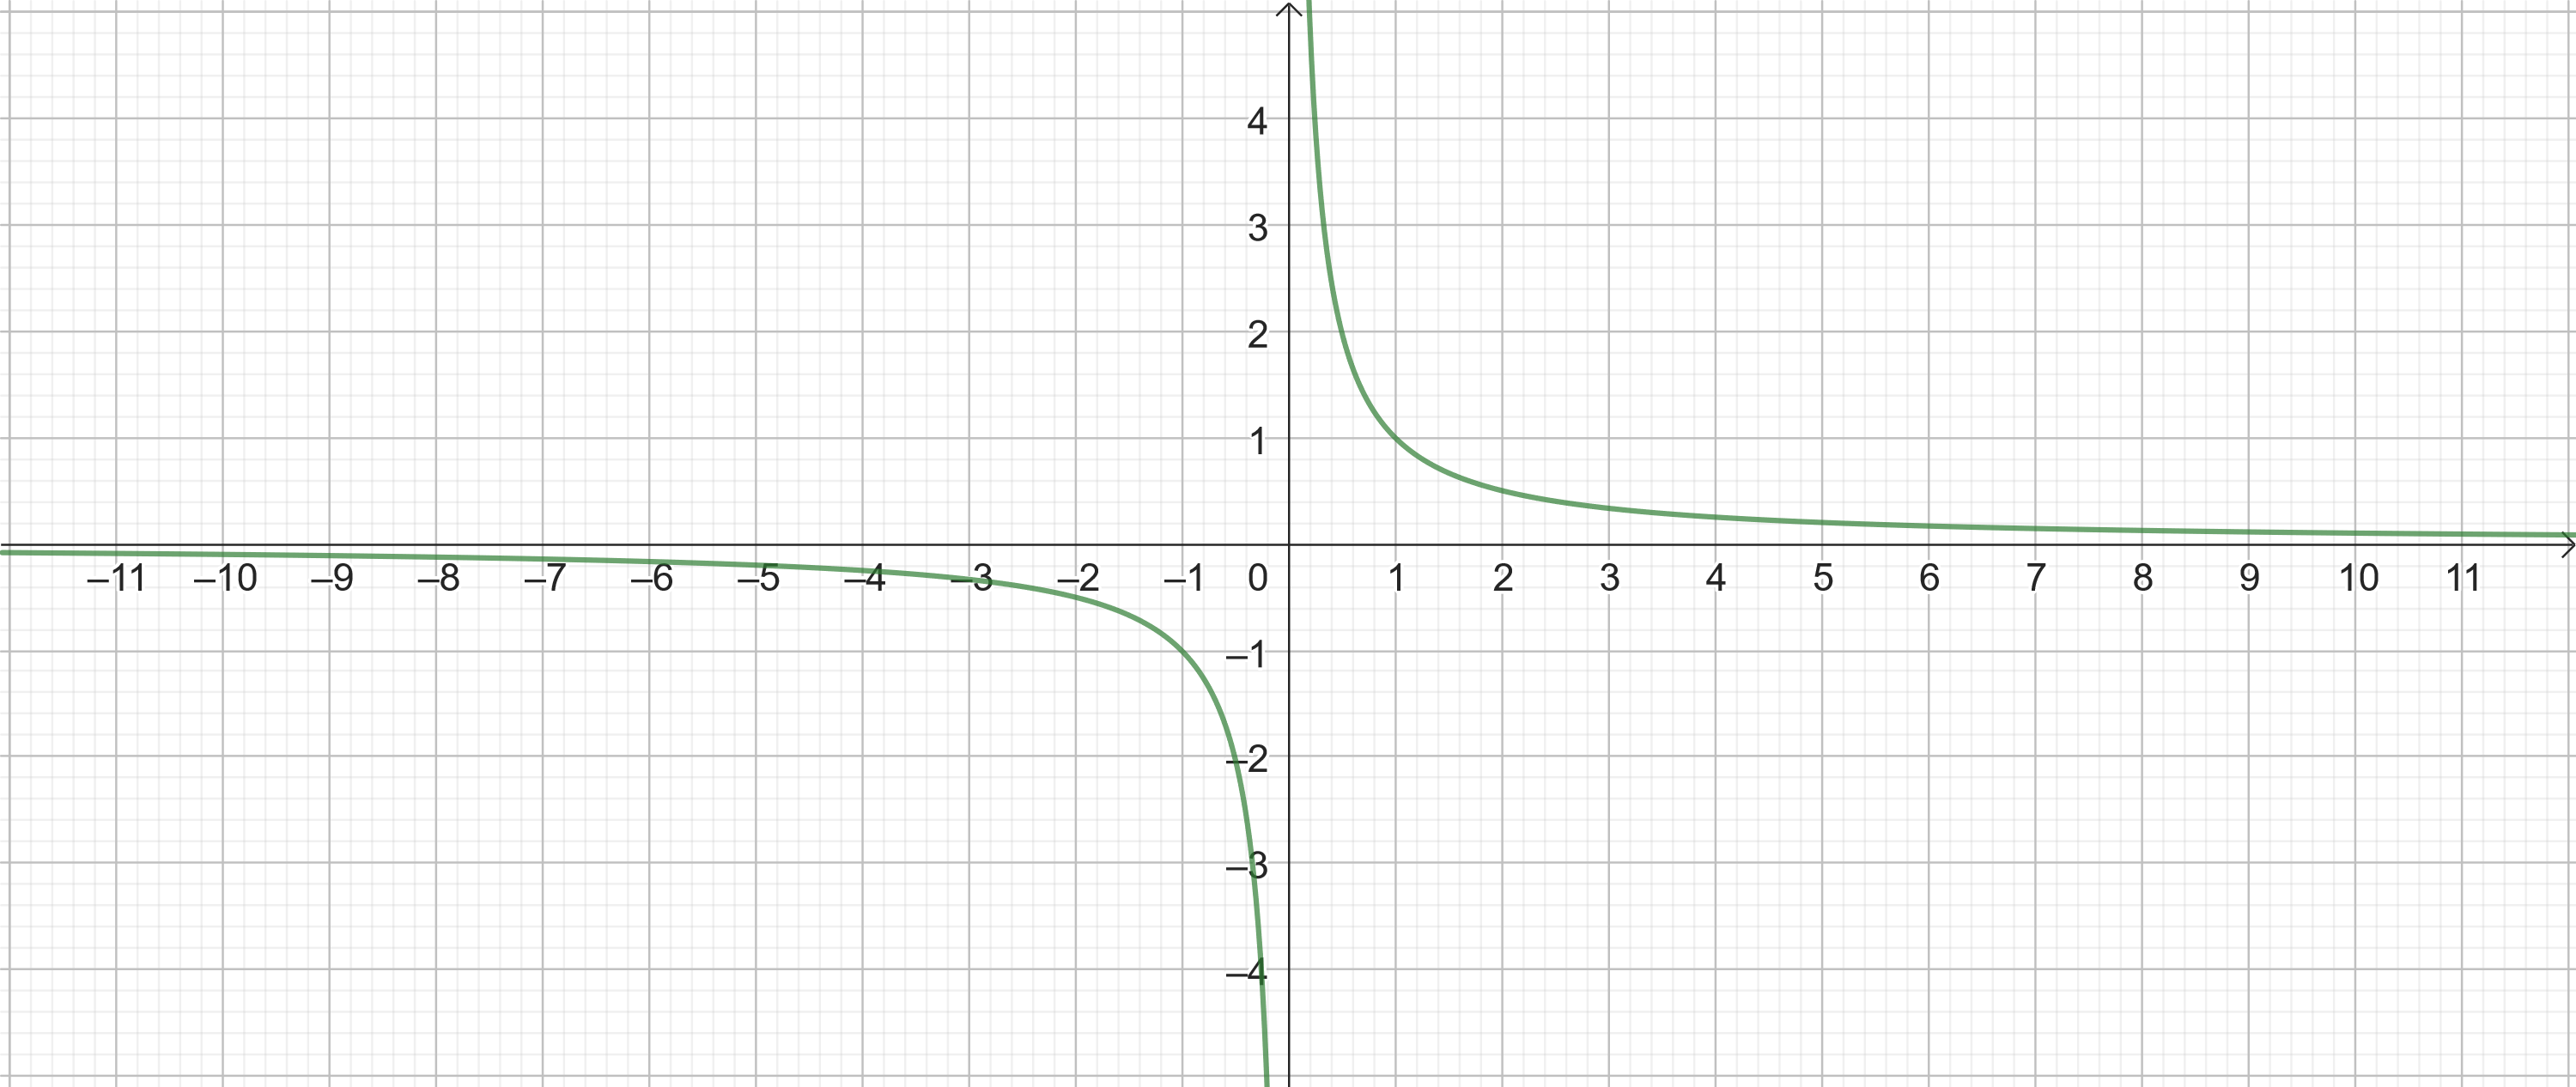
\includegraphics[width=\textwidth]{Courbe.png}
\end{center}
\end{proposition}
\section{Dérivée}
\begin{proposition}
La fonction inverse est dérivable sur $\left]-\infty;0\right[ \cup \left]0;+\infty \right[$, et sa dérivée est définie par
\begin{equation*}
x \mapsto - \dfrac{1}{x^2}
\end{equation*}
\end{proposition}
\begin{proposition}
La fonction inverse est \textbf{décroissante} sur $\left]-\infty;0\right[$, et \textbf{décroissante} sur $\left]0;+\infty \right[$.
\end{proposition}
\begin{center}
\begin{tikzpicture}
\tkzTabInit{$x$/1, Signe de $f'(x)$/1, Variations de $f$/2}{$-\infty$, $0$, $+\infty$};
\tkzTabLine{,-,d,-,};
\tkzTabVar{+ /, -D+ / /, - /};
\end{tikzpicture}
\end{center}

\end{document}